\paragraph{Mathematische Beschreibung der Forward-Propagation}
\label{sec:forward_propagation_math}
\mbox{}\\\noindent Dieser Abschnitt ist eine kurze mathematische Repräsentation des oben beschriebenen Algorithmus. Die Informationen für den gesamten Abschnitt stammen von Sven Nüesch (2023) und 3Blue1Brown (2017).

\[\sigma(x)=\frac{1}{1+e^{-x}}\]

\noindent Die Sigmoid-Funktion ist eine beliebte Aktivierungsfunktion, die die Summation der gewichteten Eingaben und des Bias in einen Wert zwischen 0 und 1 umwandelt. Diese Funktion ermöglicht es dem Netzwerk, Nichtlinearitäten zu modellieren.

\[b=Bias\]
\[w=Weight\]

\noindent Gewichte sind die Parameter, die die Stärke der Verbindung zwischen den Neuronen in aufeinanderfolgenden Schichten steuern, während der Bias eine zusätzliche Anpassung ermöglicht, die zu der gewichteten Summe der Eingaben hinzugefügt wird, um die Aktivierung eines Neurons zu beeinflussen.

\[a=Activation\]
Die Aktivierung ist die Ausgabe eines Neurons nach Anwendung der Aktivierungsfunktion auf die gewichtete Summe der Eingaben plus Bias.

\begin{figure}[H]
	\centering
		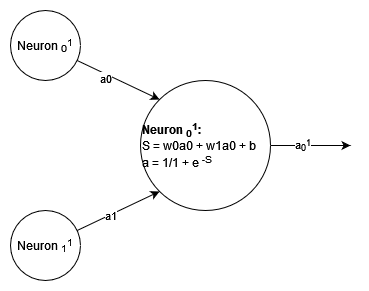
\includegraphics[width=0.5\linewidth]{nn2detail.png}
	\label{fig:nn2detail}
	\caption{Abbildung von 3 isolierten Neuronen (Inspiriert von \href{https://www.youtube.com/watch?v=aircAruvnKk}{3Blue1Brown})}
\end{figure}

\[a_{0}^{(1)} = \sigma(w_{0}\; a_{0}^{(0)} + w_{1}\; a_{1}^{(0)} + b) = \sigma(\sum_{j}^{n} w_{j}\;a_{j} ^{(0)} + b)\]

\noindent Diese Formel repräsentiert die gewichtete Summe der Eingabesignale $a_j(0)^(0)$?, wobei jedes Eingabesignal mit einem Gewicht $w_j$? multipliziert wird. Der Index $j$ läuft über alle Eingaben von 0 bis $n$, wobei $n$ die Anzahl der Eingabeneuronen ist. Zusätzlich wird ein Bias-Term $b$ hinzugefügt, der es dem Neuron ermöglicht seine Ausgabe unabhängig von der Eingabe anzupassen.

\begin{figure}[H]
	\centering
		\includegraphics[height=0.5\textheight]{nn6verknüpft.png}
	\label{fig:nn6verknüpft}
	\caption{Abbildung von einigen Neuronen (Inspiriert von \href{https://www.youtube.com/watch?v=aircAruvnKk}{3Blue1Brown})}
\end{figure}

\[a_{0}^{(1)} = \sigma(w_{0,0}\; a_{0}^{(0)} + w_{0,1}\; a_{1}^{(0)} + \cdots + w_{0,n}\; a_{n} ^{(0)} + b_{0})\]

\noindent Diese Gleichung beschreibt die Aktivierung $a_0^{(1)}$ eines Neurons in der ersten Schicht (ausser der Eingabeschicht) basierend auf den Eingaben $a_{i}^{(0)}$ (wo $i$ von $0$ bis $n$ läuft), den Gewichten $w_{0,i}$, die diese Eingaben mit dem Neuron verbinden, und dem Bias $b_0$.
\\
Um von dieser Gleichung eines einzelnen Neurons zu den Gleichungen für einen gesamten Layer mit $k+1$ Neuronen zu gelangen, erweitern wir die vorherige Gleichung für jedes Neuron $j$ im Layer:

\[a_j^{(1)}=\sigma(w_{j,0}\; a_0^{(0)} + w_{j,1}\; a_1^{(0)} + \cdots + w_{j,n}\; a_n^{(0)} + b_j)\]

\noindent Dabei läuft $j$ von $0$ bis $k$.
\\
Die Gleichungen für alle Neuronen in einem Layer können effizient in Matrixform ausgedrückt werden. Die Gewichte zwischen den Eingaben und den Neuronen im Layer können in einer Gewichtsmatrix $W$ zusammengefasst werden, die Eingaben in einem Vektor $a^{(0)}$, und die Bias-Werte in einem Bias-Vektor $b$. Die Operation wird dann als Matrix-Vektor-Multiplikation dargestellt:

\[\sigma(\left(\begin{array}{c} w_{0,0}\; w_{0,1}\! \cdots\; w_{0,n} \\ w_{1,0}\; w_{1,1}\; \cdots\; w_{1,n} \\ \vdots\quad  \vdots\quad  \ddots\quad  \vdots \\ w_{k,0}\; w_{k,1}\; \cdots\; w_{k,n}  \end{array}\right) \left(\begin{array}{c} a_{0} ^{(0)} \\ a_{1}^{(0)} \\ \vdots \\ a_{n}^{(0)} \end{array}\right) + \left(\begin{array}{c} b_{0} \\ b_{1} \\ \vdots \\ b_{n} \end{array}\right))\]

\noindent Hier repräsentiert $W$ die Gewichtsmatrix, $a^{(0)}$ den Eingabevektor (aus der vorherigen Schicht), und $b$ den Bias-Vektor. Die Aktivierungsfunktion $\sigma$ wird elementweise auf das Ergebnis der Matrix-Vektor-Addition angewendet.
\\
Schliesslich kann die obige Gleichung noch weiter vereinfacht werden, indem die Matrix, der Eingabevektor und der Bias-Vektor einfach durch ihre Symbole dargestellt werden, ohne ihre Elemente explizit aufzuführen. Dies führt zur kompaktesten Form:

\[a^{(1)} = \sigma(W\; a^{(0)} + b)\]

\noindent In dieser Gleichung steht $a^{(1)}$ für den Vektor der Aktivierungen der Neuronen im betrachteten Layer nach Anwendung der Aktivierungsfunktion auf die gewichtete Summe der Eingaben und der Bias-Werte.
